\chapter[Referencial Teórico]{Referencial Teórico}

\section{Fenômenos de Transporte de Calor}

A transferência de calor é um fenômeno em que, na física, dois corpos com temperaturas diferentes trocam suas energias térmicas quando estão em contato ou em um mesmo ambiente, para que atinjam o equilíbrio.

Alguns materiais são isolantes térmicos e tendem a evitar transferência. São importantes para prevenir gasto energético desnecessário e manter sistemas sem troca de calor se necessário.

Para o projeto proposto, é necessário uma temperatura interna entre 2 e 4 graus Celsius para preservar as características desejadas e não danificar o órgão colocado. Além disso, a caixa deve ser isolada termicamente para que minimize ao máximo as trocas de calor e não afete o órgão transportado.

Essa transferência de calor pode ser classificada de três formas diferentes: Condução, convecção e radiação.

\subsection{Condução}
Ocorre entre corpos que estão em contato físico e está relacionada com a energia cinética, a colisão entre os átomos realiza a transferência de energia cinética (calor) para as moléculas próximas. Com isso, o calor flui do local com temperaturas mais altas para o local com temperatura mais baixa.

A facilidade com que o calor transferido pode ser medido através da condutividade, normalmente, sólidos conduzem melhor que líquidos, e líquidos conduzem melhor do que sólidos.

\begin{table}[H]
\centering
\begin{tabular}{|c|c|}
\cline{1-2}
Material               & Condutibilidade Térmica (k) \\ \cline{1-2}
Cobre (puro)           & 339                         \\ \cline{1-2}
Ouro (puro)            & 317                         \\ \cline{1-2}
Alumínio (puro)        & 237                         \\ \cline{1-2}
Ferro (puro)           & 80,2                        \\ \cline{1-2}
Aço Carbono (1\%)      & 43                          \\ \cline{1-2}
Aço Inoxidável (18/18) & 15,1                        \\ \cline{1-2}
Vidro                  & 0,81                        \\ \cline{1-2}
Plásticos              & 0,2 -- 0,3                  \\ \cline{1-2}
Água (liquido)         & 0,6                         \\ \cline{1-2}

\end{tabular}
\caption{Condutividade térmica dos materiais a 300K. Fonte: BENNETT, 2008}
\label{condutividade térmica}
\end{table}

\subsection{Convecção}

A convecção ocorre em líquidos ou gases somente. Ocorre pela diferença de densidades, o ar frio é mais denso e tom ao lugar do ar quente, o ar frio lentamente ganha calor e realiza o ciclo novamente.

Existem dois tipos de convecção: a natural (explicada acima) e a forçada, a qual utiliza aspiradores e bombas para fazer o deslocamento do fluído. (BENNETT, 2008; TIPLER, 2009).

\subsection{Radiação}

São ondas eletromagnéticas que se movem na velocidade da luz, por ser a única capaz de percorrer o espaço, é a principal maneira de transferência de calor do Sol com o planeta terra.

\begin{figure}[H]
\centering
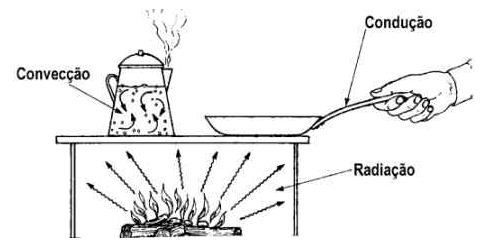
\includegraphics[width=8cm]{figuras/transferenciadecalor.png}
\caption{Mecanismos de transferência de calor}
\end{figure}

\section{Calorimetria}
A calorimetria é o estudo do calor como energia térmica em trânsito. Com dois corpos em temperaturas diferentes, a transmissão ocorre do corpo mais quente para o mais frio até atingirem o equilíbrio térmico. Uma das medidas mais usadas é a quantidade de calor (Q), ao receber energia térmica, essa quantidade de calor é positiva, ao perder é negativa.

\subsection{Calor Sensível e Latente}
Um corpo pode receber dois tipos de calor, o latente e o sensível. O calor latente é obtido quando o corpo muda de estado físico por causa dessa transferência, já o calor sensível é apenas mudança na temperatura do corpo.

Podemos representar seus cálculos com a fórmula fundamental da calorimetria e a equação para calcular o calor latente. Que são:

\begin{align}
Q_S=m \cdot c \cdot \Delta T
\end{align}
\begin{align}
Q_L=m \cdot L
\end{align}

Onde:
\begin{itemize}
\item $Q_S$ = Quantidade de calor sensível (em joules)
\item m = Massa do corpo em gramas
\item c = Calor sensível
\item $\Delta$T = Diferença de temperatura em ºC
\item $Q_L$ = Quantidade de calor Latente (em joules)
\item L = Constante de calor latente
\end{itemize}

\section{Fenômenos termoelétricos}
A termoelétrica estuda esses fenômenos que associam corrente elétrica com geração de energia elétrica ou térmica. É possível criar uma corrente elétrica e usar essa corrente para controlar um fluxo de aquecimento.

Alguns dos usos mais comuns de um dispositivo termoelétrico são telecomunicações, conversão de energia, fontes alternativas e refrigeração. Podem ter baixa eficiência em metais (mesmo sendo bons condutores térmicos e elétricos), e alta eficiência em semicondutores.

Temos 3 tipos de efeitos termoelétricos, que são efeito de Peltier, de Seebeck e de Thomson.

\subsection{Efeito Seebeck}
O físico , Thomas Johann Seebeck em 1821 uniu dois matérias condutores ou semicondutores, de diferentes temperaturas, com uma junta de medição, ocorre o aparecimento de uma diferença de potencial que gera uma corrente elétrica. 

Esse princípio é utilizado em termopares, um sensor de temperatura usado com frequência ainda hoje. 

\subsection{Efeito de Peltier}
Em 1834, o físico francês Jean Charles Athanase Peltier conseguiu observar o inverso do feito de Seebeck, que foi chamado de efeito de Peltier.

Aplicando uma tensão em um circuito elétrico fechado que gera uma corrente que atravessa o corpo formado por condutores ou semicondutores, absorve e libera calor em suas junções, que podem ser trocadas com mudança da direção da corrente.

\begin{figure}[H]
\centering
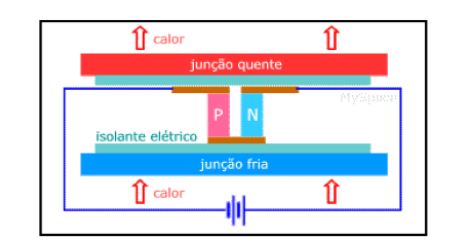
\includegraphics[width=10cm]{figuras/efeitopeltier.png}
\caption{Representação esquemática da célula de Peltier}
\end{figure}

Para a junção quente, a corrente elétrica flui do lado positivo para o lado negativo e para a junção fria, a corrente elétrica flui do lado negativo para o positivo. 

A transferência do fluxo de calor para os elementos P e N se dá da seguinte forma: O elemento positivo P absorve calor elevando seu nível de energia que o faz migrar para o lado quente que possui uma menor quantidade de energia. Através de ventiladores, coolers e dissipadores, retira-se calor desse elemento que retorna ao lado P reiniciando o ciclo. (COSTA 2010; SOUZA, 2011; MARQUES, 2011).

\subsection{Efeito Thompson}
Mais tarde foi William Thompson na Irlanda que descobriu que dependendo do sentido da corrente elétrica poderia poderia produzir frio ou calor.

\begin{figure}[H]
\centering
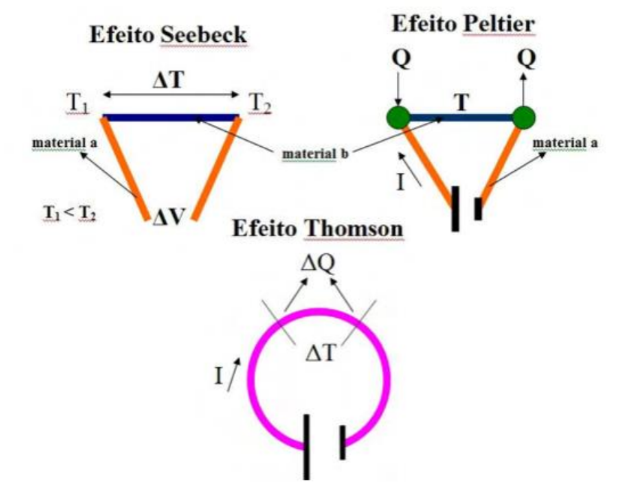
\includegraphics[width=8cm]{figuras/efeitothompson.png}
\caption{Esquema dos efeitos de Peltier, Seebck e Thompson}
\end{figure}

\section{Célula de Peltier}

A célula de peltier é uma pastilha termoelétrica muito usada na area da eletronica, automotiva, militar e industrial. Suas principais vantagens sao o fácil controle do calor liberado, baixo custo, não libera gás fréon, tamanho reduzido e boa durabilidade.

Para entender melhor o funcionamento de uma pastilha peltier temos a seguinte imagem.

\begin{figure}[H]
\centering
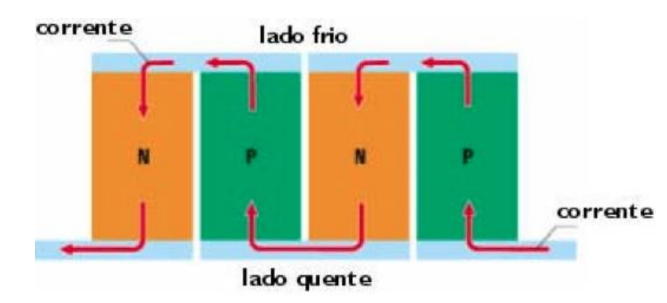
\includegraphics[width=8cm]{figuras/peltier1.png}
\caption{Esquema do caminho da corrente na célula de Peltier}
\end{figure}

A célula é formada por semicondutores de tipo N e P e a corrente caminha de acordo com a imagem.

As faces das célula são formadas por material cerâmico, o que ajuda no isolamento e na condutibilidade térmica. Quando aplicamos uma diferença de potencial, de acordo com o efeito de Peltier, é gerada uma corrente corrente que cria um gradiente de temperatura entre as faces.

Alguns cuidados devem ser tomados ao montar uma placa de Peltier, a utilização de coolers o ventiladores é essencial para que não ocorra o superaquecimento das células o esquema da imagem a seguir também é recomendado, inclusive utilizando uma pasta térmica para otimizar a transferência de calor.

\begin{figure}[H]
\centering
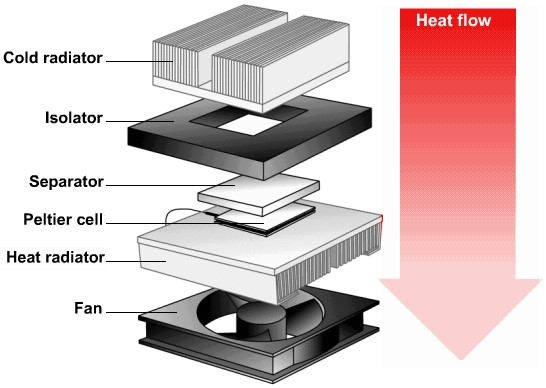
\includegraphics[width=8cm]{figuras/peltier2.jpg}
\caption{Esquema de montagem da célula de Peltier}
\end{figure}

Outro cuidado é observar a quantidade de calor máximo que a pastilha escolhida pode transferir ao aplicar seu potencial e corrente máximos, o que produzirá a maior diferença de temperatura. 

Um método para aumentar a transferência de calor é colocar mais de uma pastilhas uma sobre a outra,chamado de multi-estágios, a parte quente de uma das pastilhas na parte fria da outra. Porém a diferença de temperatura não pode passar de 60 graus Celsius.

\begin{figure}[H]
\centering
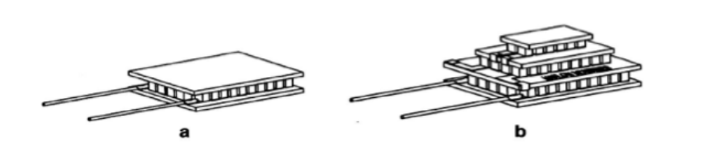
\includegraphics[width=8cm]{figuras/peltier3.png}
\caption{Célula em estágio simples (a) e multi-estágios (b)}
\end{figure}

\section{Modelo cliente-servidor/sistema web}

Em um modelo cliente-servidor, os dados de um sistema são armazenados em poderosos computadores chamados servidores. Os usuário utilizam máquinas mais simples, chamadas de clientes. As máquinas cliente e servidor são conectadas entre si por uma rede, conforme ilustrado pela Fig. \ref{cliente_servidor}.

\begin{figure}[H]
\centering
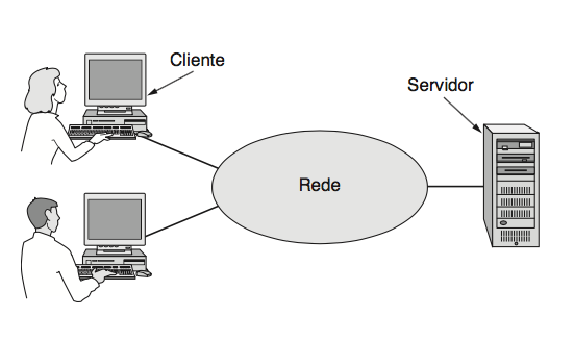
\includegraphics[width=8cm]{figuras/cliente_servidor.eps}
\caption{Modelo cliente-servidor.}\label{cliente_servidor}
\end{figure}

Em uma aplicação web, o servidor fornece páginas Web com base em seu banco de dados em resposta a solicitação do cliente. Sob a maioria das condições, um único servidor pode lidar com um grande número (centenas ou milhares) de clientes simultaneamente.

Examinando o modelo cliente-servidor em detalhes, é possível perceber que existem dois processos em execução, um na máquina cliente e outro na máquina servidor. A comunicação toma a forma do processo cliente enviando uma mensagem pela rede ao processo servidor. Então, o processo cliente espera por uma mensagem de resposta. Quando processo servidor recebe a solicitação, ele executa o trabalho solicitado ou procura pelos dados solicitados e envia uma resposta de volta (Fig. ) (TENENBAUM, 2011).

\begin{figure}[H]
\centering
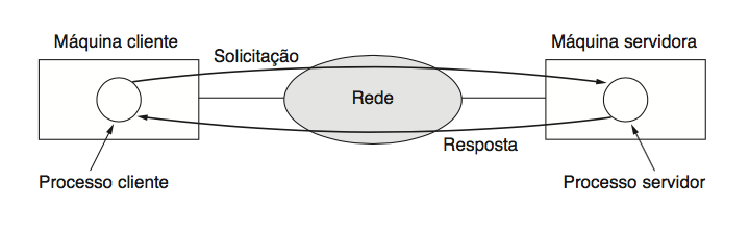
\includegraphics[width=10cm]{figuras/cliente_servidor_mensagens.eps}
\caption{Mensagens trocadas entre um processo cliente e um processo servidor}
\end{figure}

\section{Framework Django}

Django é um framework gratuito e de código aberto para a criação de aplicações web, escrito em Python, uma linguagem de programação multiparadigma. É um framework web, ou seja, é um conjunto de componentes que ajuda a desenvolver sites de forma mais rápida e mais fácil.

Quando se está construindo um site, o desenvolvedor sempre precisa de um conjunto similar de componentes: uma maneira de lidar com a autenticação do usuário (inscrever-se, realizar login, realizar logout), painel de gerenciamento para o seu site, formulários, upload de arquivos, etc. Há muito tempo, outras pessoas notaram várias semelhanças nos problemas enfrentados pelos desenvolvedores web quando estão criando um novo site, então eles uniram-se e criaram os frameworks (Django é um deles) que lhe dão componentes prontos, que você pode usar. O framework Django utiliza o padrão MTV (model-template-view), onde as views funcionam como controllers e templates funcionam como views. 

\section{Sistema interno}

Sistema responsável por se comunicar com o aparato eletrônico, recebendo dados e interpretá-los. Para isso, será utilizado a linguagem de programação C++. C++ é uma linguagem de programação de alto nível com facilidades para o uso em baixo nível. Foi desenvolvida por Bjarne Stroustrup (foto) como uma melhoria da linguagem C, e desde os anos 1990 é uma das linguagens mais populares do mundo.

Alguns profissionais afirmam que C++ é a linguagem mais poderosa que existe, veja algumas características dela:

\begin{itemize}
\item É um superconjunto da linguagem C, e contém vários melhoramentos;
\item É a porta para a programação orientada a objetos;
\item C++ pode virtualmente ser efetivamente aplicado a qualquer tarefa de programação;
\item Há vários compiladores para diversas plataformas tornando a linguagem uma opção para programas multiplataforma.
\end{itemize}







\section{Ergonomia de carregamento de peso}

Para uma pessoa de 18 a 35 anos, os limites de pesos que podem ser levantados sem causar problemas à sua saúde são 40 kg para homens e 20 kg para mulheres. Portanto em média 30 kg por pessoa. Deste modo, um objeto carregado por duas pessoas poderia pesar um máximo de 60 kg. Aplicando um fator de segurança de 30\%, o peso máximo para um objeto carregado por duas pessoas é aproximadamente 40 kg.

\section{TERMOVIDA – Caixa térmica para transporte de órgãos para transplantes}

O projeto TERMOVIDA consiste em uma caixa térmica para transporte de órgãos para transplantes com um sistema de refrigeração autônoma.

A legislação da ANVISA regulamenta como deve se dar o transporte de órgãos para transplante, as informações que devem ser coletadas que constatam o tempo de vida e a temperatura ideal a ser mantida para que os órgãos que sejam transportados em segurança por este dispositivo puderam indicar como deve ser o recipiente e quais sao os equipamentos necessário para que o mesmo funcione corretamente.

Neste projeto, é utilizada uma pastilha de efeito Peltier para a refrigeração da caixa, controlada por histerese, via um micro-controlador. O equipamento, utilizado durante o transporte em veículos, utiliza alimentação elétrica do sistema de 12V do veículo.

A estrutura da caixa é feita de material isolante térmico. Esta possui uma porta de ventilação na lateral, onde está posicionada a pastilha Peltier, e um espaço no qual um painel LCD sensível ao toque está alocado. O painel é responsável por mostrar as condições monitoradas.

\begin{figure}[H]
\centering
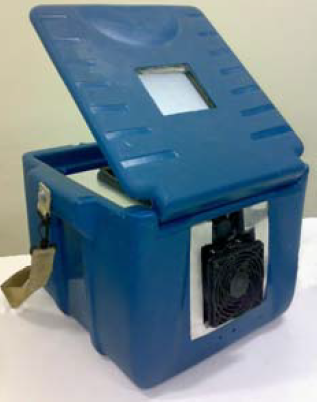
\includegraphics[scale=1]{figuras/termovida.png}
\caption{TERMOVIDA - Caixa térmica para transporte de órgãos para transplantes}
\end{figure}
